\chapter{Dinamica del corpo rigido}
Consideriamo un punto materiale con posizione
\[
\underline{x}(t)=\bigl(x(t),y(t),z(t)\bigr).
\]

Per avere una forma analitica di $\underline{x}(t)$ dobbiamo passare dalla legge di Newton
\[
m\,\ddot{\underline{x}}=\underline{f}\bigl(\underline{x},\dot{\underline{x}},t\bigr),
\]
Dato un corpo dotato di massa inerziale $m$ quest'ultima è quindi la costante di proporzionalità tra accelerazione e risultante delle forze.

\begin{oss}{}
$\underline{f}$ non dipende mai da $\ddot{\underline{x}}$. Questa è un'evidenza fisica.
\end{oss}

Consideriamo un insieme di $n$ punti materiali. Per ogni punto possiamo scrivere
\[
m_i\,\ddot{\underline{x}}_i=\underline{f}_i\bigl(x_1,\dots,x_n,\dot{x}_1,\dots,\dot{x}_n,t\bigr).
\]

\begin{oss}{}
Nelle $\{\underline{f}_i\}$ sono comprese anche le forze vincolari, che pur non essendo funzioni esplicite di
\[
(x_1,\dots,x_n,\dot{x}_1,\dots,\dot{x}_n,t),
\]
ne dipendono comunque in maniera implicita.
\end{oss}\begin{example}{}
Consideriamo un sistema di $3$ punti materiali vincolati attraverso due aste rigide di lunghezza $d_1,d_2$ e due molle di rigidezza $K_1,K_2$, disposti come in figura.

\begin{figure}
\centering
\begin{tikzpicture}[scale=1.1, >=Latex]

% assi
\draw[->] (-0.3,0) -- (5.6,0) node[right] {$y$};
\draw[->] (0,-0.3) -- (0,3.8) node[above] {$z$};
\draw[->] (0,0) -- (-1.0,-1.0) node[below] {$x$};

% punti
\coordinate (O) at (0,0);
\coordinate (P1) at (1.2,2.2);
\coordinate (P2) at (3.0,2.2);
\coordinate (P3) at (4.3,1.4);
\coordinate (P4) at (2.5,0);

% punti materiali
\fill (P1) circle (2pt) node[above left] {$1$};
\fill (P2) circle (2pt) node[above] {$2$};
\fill (P3) circle (2pt) node[right] {$3$};
\fill (P4) circle (2pt) node[below] {$4$};

% molla K1 tra O e P1
\draw[decorate, decoration={coil, aspect=0.45, segment length=4pt, amplitude=3pt}]
  (O) -- (P1);
\node[left] at (0.55,1.3) {$K_1$};

% asta rigida d1 tra P1 e P2
\draw[thick] (P1) -- (P2);
\node[above] at (2.1,2.2) {$d_1$};

% molla K2 tra P2 e P3
\draw[decorate, decoration={coil, aspect=0.45, segment length=4pt, amplitude=3pt}]
  (P2) -- (P3);
\node[right] at (3.55,2.0) {$K_2$};

% asta rigida d2 tra P4 e P3
\draw[thick] (P4) -- (P3);
\node[below right] at (3.35,0.75) {$d_2$};


% nota punto 4
\node[below right] at (2.7,-0.45) {$4$ fissato ed esterno al sistema};

\end{tikzpicture}
\end{figure}

Imponiamo il vincolo olonomo
\[
\lvert \underline{x}_1-\underline{x}_2\rvert=d_1=\text{cost}.
\]
Come tutti i vincoli olonomi, esso comporta una reazione vincolare, cioè una forza incognita che permette il soddisfacimento del vincolo.

Allo stesso modo imponiamo
\[
\lvert \underline{x}_3-\underline{x}_4\rvert=d_2=\text{cost}.
\]

Detta $\underline{f}_i$ la risultante delle forze agenti sul punto $i$-esimo, abbiamo
\[
\underline{f}_1=-K_1(\underline{x}_1-\underline{0})+\underline{f}_{12},
\]
dove $-K_1(\underline{x}_1-\underline{0})$ è una forza attiva esterna, mentre $\underline{f}_{12}$ è una forza interna vincolare.

Inoltre
\[
\underline{f}_2=\underline{f}_{21}-K_2(\underline{x}_2-\underline{x}_3),
\]
dove $\underline{f}_{21}$ è una forza interna vincolare, mentre $-K_2(\underline{x}_2-\underline{x}_3)$ è una forza attiva interna.

Infine
\[
\underline{f}_3=-K_2(\underline{x}_3-\underline{x}_2)+\underline{f}_{34},
\]
dove $-K_2(\underline{x}_3-\underline{x}_2)$ è una forza attiva interna, mentre $\underline{f}_{34}$ è una forza esterna vincolare.

Notiamo che
\[
\underline{f}_{23}=-K_2(\underline{x}_2-\underline{x}_3)
              =K_2(\underline{x}_3-\underline{x}_2)
              =-\underline{f}_{32},
\]
quindi tali forze soddisfano il principio di azione e reazione.
\end{example}

\begin{example}{}
Descriviamo la dinamica di un moto piano di un punto. Imponiamo il vincolo
\[
z_P=0.
\]

\begin{figure}
\centering
\begin{tikzpicture}[scale=1.1, >=Latex]
  % piano vincolante
  \draw (-2.2,0) -- (3.2,0);
  \draw (-1.0,1.6) -- (3.2,1.6);
  \draw (-2.2,0) -- (-1.0,1.6);

  % punto P
  \fill (0.2,0.8) circle (2pt) node[right] {$P$};

  % asse verticale delle forze
  \draw[->] (0.2,0.8) -- (0.2,2.0);
  \node[right] at (0.2,1.85) {$\underline{R}$};

  \draw[->] (0.2,0.8) -- (0.2,-0.4);
  \node[right] at (0.2,-0.25) {$m\underline{g}$};
\end{tikzpicture}
\end{figure}

Se
\[
m\,\ddot{\underline{x}}_P=0,
\]
allora c'è una forza esterna vincolare $\underline{R}$ dovuta al vincolo $z_P=0$ che annulla $m\underline{g}$, ovvero
\[
\underline{R}=m\underline{g}.
\]
\end{example}

\section{Prima equazione cardinale del moto di un corpo rigido}
Consideriamo un sistema di $n$ particelle caratterizzate ognuna da una posizione $\underline{x}_i$ e da una massa $m_i$.

\begin{definition}{}
Si dice centro di massa del sistema
\[
\underline{x}_G = \frac{\sum_{i=1}^{n} m_i \,\underline{x}_i}{\sum_{i=1}^{n} m_i}.
\]
\end{definition}

\begin{definition}{}
Si dice vettore posizione del punto $i$-esimo rispetto al centro di massa
\[
\underline{x}_i' = \underline{x}_i - \underline{x}_G.
\]
\end{definition}

\begin{figure}[H]
\centering
\begin{tikzpicture}[scale=1.2, >=Latex]

% assi 3D
\draw[->] (-1.0,0,0) -- (3.0,0,0) node[right] {$x$};
\draw[->] (0,-1.0,0) -- (0,3.0,0) node[above] {$y$};
\draw[->] (0,0,-1.0) -- (0,0,3.0) node[above] {$z$};

% punti e vettori
\coordinate (O) at (0,0,0); % origine
\coordinate (X1) at (2,2,1);  % primo punto
\coordinate (X2) at (1.5,3,2); % secondo punto

% vettori
\draw[->,red] (O) -- (X1) node[midway, below right] {$\underline{x}_i$}; % vettore x1
\draw[->,blue] (O) -- (X2) node[midway, above right] {$\underline{x}_G$}; % vettore x2

% vettore differenza
\draw[->,green] (X2) -- (X1) node[midway, above right] {$\underline{x}_i'$}; % differenza tra i vettori

\end{tikzpicture}
\end{figure}

\begin{oss}{}
\[
\sum_{i=1}^{n} m_i \,\underline{x}_i' = \sum_{i=1}^{n} m_i \,(\underline{x}_i - \underline{x}_G) = \sum_{i=1}^{n} m_i \, \underline{x}_i - \sum_{i=1}^{n} m_i \,\underline{x}_G
\]
\[
\underline{x}_G'
=
\frac{\sum_{i=1}^{n} m_i \underline{x}_i'}{\sum_{i=1}^{n} m_i}
=
\frac{\sum_{i=1}^{n} m_i(\underline{x}_i-\underline{x}_G)}{\sum_{i=1}^{n} m_i}
\]
\[
=
\frac{\sum_{i=1}^{n} m_i \underline{x}_i}{\sum_{i=1}^{n} m_i}
-
\frac{\sum_{i=1}^{n} m_i \underline{x}_G}{\sum_{i=1}^{n} m_i}
=
\underline{x}_G-\underline{x}_G
=
\underline{0}
\]

Questo è ovvio perché la posizione del centro di massa calcolato in un sistema di riferimento che ha l'origine nel centro di massa è l'origine stessa.
\end{oss}

Consideriamo il sistema di $n$ punti materiali di posizioni $\underline{x}_i$ e masse $m_i$ sottoposti a forze di risultante $\underline{f}_i$. Allora per ogni punto vale:
\[
m_i \underline{\ddot{x}}_i = \underline{f}_i.
\]
Sommiamo su tutti i punti:
\[
\sum_{i=1}^{n} m_i \underline{\ddot{x}}_i = \sum_{i=1}^{n} m_i \frac{d^2}{dt^2} \left( \underline{x}_G + \underline{x}_i' \right) = \frac{d^2}{dt^2} \left( \sum_{i=1}^{n} m_i \underline{x}_G + \sum_{i=1}^{n} m_i \underline{x}_i' \right)
\]

\[
= m \frac{d^2}{dt^2} \underline{x}_G = \frac{d}{dt} \left( m \underline{v}_G \right)
\]

Ora, dette $\underline{f}_i^{\text{est}}$ e $\underline{f}_i^{\text{int}}$ rispettivamente la risultante delle forze esterne che agiscono su $i$ e la risultante delle forze interne che agiscono su $i$, possiamo scrivere:
\[
\underline{f}_i = \underline{f}_i^{\text{est}} + \underline{f}_i^{\text{int}} = \underline{f}_i^{\text{est}} + \sum_{\substack{j=1 \\ j \neq i}}^{n} \underline{f}_{ij}
\]
Allora otteniamo
\[
\sum_{i=1}^{n} m_i \underline{\ddot{x}}_i = \sum_{i=1}^{n} \underline{f}_i = \sum_{i=1}^{n} \underline{f}_i^{\text{est}} + \sum_{i=1}^{n} \sum_{\substack{j=1 \\ j \neq i}}^{n} \underline{f}_{ij} = \sum_{i=1}^{n} \underline{f}_i^{\text{est}}
\]
Dal momento che $\sum_{i=1}^{n} \sum_{\substack{j=1 \\ j \neq i}}^{n} \underline{f}_{ij} = \underline{0}$ per il principio di azione e reazione (le forze interne si annullano a due a due!).\\
Otteniamo infine
\[
\frac{d}{dt} \left( m \underline{v}_G \right) = \sum_{i=1}^{n} \underline{f}_i^{\text{est}}.
\]
detta \textbf{prima equazione cardinale del moto di un corpo rigido.}

\begin{oss}{}
Il centro di massa di un corpo rigido si comporta come un punto materiale sottoposto solo alle forze esterne.
\end{oss}


\begin{example}{}
    Considero un disco piano che si muove di moto di puro strisciamento con il suo centro vincolato ad una molla orizzontale.

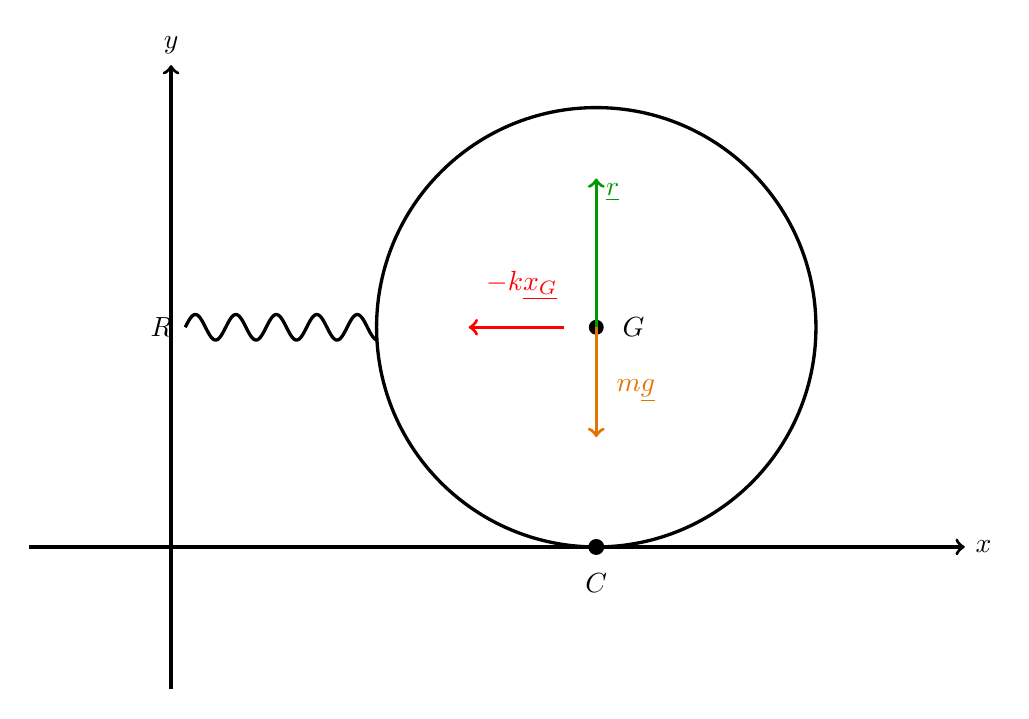
\begin{tikzpicture}[scale=0.9]
  % assi
  \draw[very thick, ->] (-2,0) -- (11.2,0) node[right] {$x$};
  \draw[very thick, ->] (0,-2) -- (0,6.8) node[above] {$y$};

  % disco
  \draw[very thick] (6,3.1) circle (3.1);

  % punto di contatto C
  \fill (6,0) circle (3.2pt);
  \node[below=6pt] at (6,0) {$C$};

  % centro G
  \fill (6,3.1) circle (3pt);
  \node[right=6pt] at (6,3.1) {$G$};

  % molla orizzontale verso l'asse y
  \draw[very thick]
    plot[smooth, samples=200, domain=0:2.7]
    ({0.2+\x},{3.1 + 0.18*sin(deg(11*\x))});
  \node[left] at (0.15,3.1) {$R$};

  % forza elastica
  \draw[red, very thick, ->] (5.55,3.1) -- (4.2,3.1);
  \node[red, above] at (4.95,3.35) {$-k\underline{x_G}$};

  % reazione vincolare r
  \draw[green!60!black, very thick, ->] (6,3.1) -- (6,5.2);
  \node[green!60!black, right] at (6,5.0) {$\underline{r}$};

  % peso mg
  \draw[orange!90!black, very thick, ->] (6,3.1) -- (6,1.55);
  \node[orange!90!black, right] at (6.15,2.2) {$m\underline{g}$};
\end{tikzpicture}

I vincoli sono quindi
\[
\dot{x}_C = 0 \quad x_C = x_G
\]
che portano il sistema ad un grado di libertà. Ai vincoli è associata una forza vincolare $\underline{r}$, inoltre possiamo far confluire tutta la massa nel centro di massa e applicare lì la forza peso
\[
m\underline{g} = \sum_{i=1}^m m_i \underline{g}.
\]
Abbiamo quindi
\[
m \underline{\ddot{x}_G} = -k \underline{x_G} + \underline{r} + m\underline{g}
\]
e dal momento che
\[
\underline{\ddot{x}_G} = \ddot{x}_G \hat{i} \quad \text{e} \quad -k \underline{x_G}= -k x_G \hat{i}
\]
allora necessariamente
\[
\underline{r} = -m\underline{g}.
\]
\end{example}

\begin{oss}{}
In generale non è possibile disaccoppiare traslazione del centro di massa e rotazione.

\begin{center}
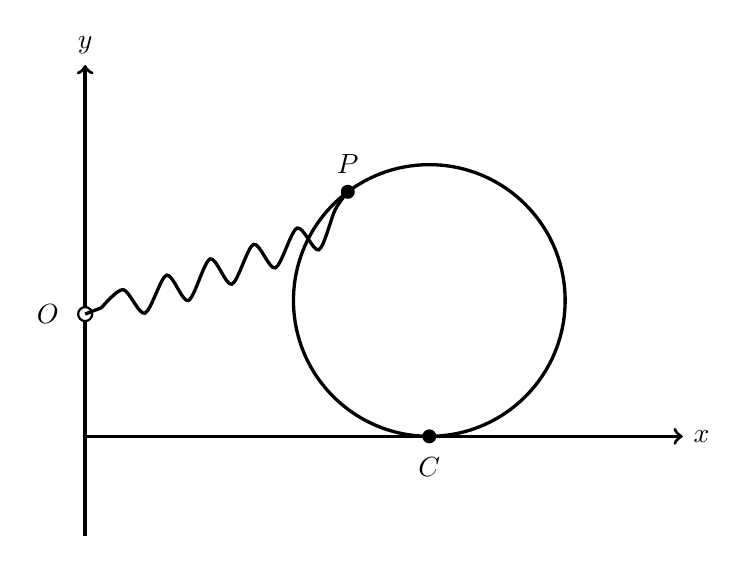
\begin{tikzpicture}[scale=1.15]
  % assi
  \draw[very thick,->] (0,-1.1) -- (0,4.1) node[above] {$y$};
  \draw[very thick,->] (0,0) -- (6.6,0) node[right] {$x$};

  % disco
  \def\R{1.5}
  \coordinate (G) at (3.8,1.5);
  \coordinate (C) at (3.8,0);
  \coordinate (O) at (0,1.35);
  \coordinate (P) at (2.9,2.7);

  \draw[very thick] (G) circle (\R);

  % punti
  \filldraw[fill=white,draw=black,line width=0.8pt] (O) circle (2.2pt);
  \node[left=6pt] at (O) {$O$};

  \fill (P) circle (2.2pt);
  \node[above=3pt] at (P) {$P$};

  \fill (C) circle (2.2pt);
  \node[below=4pt] at (C) {$C$};

  % molla
  \draw[very thick]
    (O) -- (0.18,1.42)
    plot[smooth] coordinates {
      (0.18,1.42) (0.42,1.62) (0.66,1.36) (0.90,1.78)
      (1.14,1.50) (1.38,1.96) (1.62,1.68) (1.86,2.12)
      (2.10,1.86) (2.34,2.30) (2.58,2.06) (2.76,2.50)
      (2.90,2.70)
    };
\end{tikzpicture}
\end{center}

Rilassando il moto di puro strisciamento imponendo solo
\[
y_C^{\text{Disco}}=0
\]
istantaneamente e considerando il caso in cui la molla non è orizzontale si ottiene
\[
m\ddot{\underline{x}}_G=\underline{f}^{\mathrm{ext}}=-k\bigl(\underline{x}_P-\underline{x}_O\bigr)
\]
che dipende da \(\underline{\omega}\) dal momento che \(\underline{x}_P\) dipende da \(\underline{\omega}\) attraverso
\[
\underline{v}_P=\underline{v}_C+\underline{\omega}\wedge\bigl(\underline{x}_P-\underline{x}_C\bigr).
\]
\end{oss}


\begin{example}{}
Consideriamo un sistema costituito da una persona su una barca e dalla barca. Supponiamo inizialmente che sia la barca che la persona siano fermi rispetto ad un sistema di riferimento fisso posto sulla superficie dell'acqua. Inoltre sul sistema non agisce una risultante non nulla di forze esterne.

\begin{center}
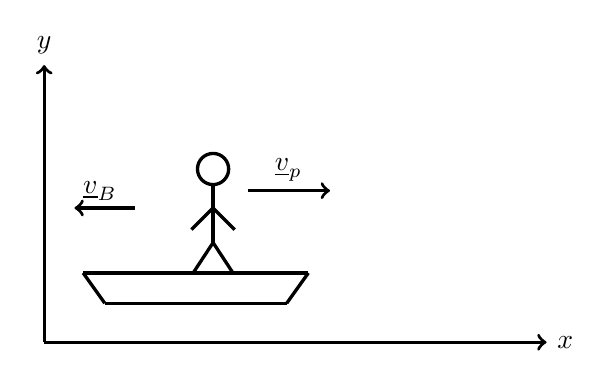
\begin{tikzpicture}[scale=1.1]
  % assi
  \draw[very thick,->] (0,0) -- (5.8,0) node[right] {$x$};
  \draw[very thick,->] (0,0) -- (0,3.2) node[above] {$y$};

  % barca
  \draw[very thick] (0.45,0.8) -- (3.05,0.8);
  \draw[very thick] (0.70,0.45) -- (2.80,0.45);
  \draw[very thick] (0.45,0.8) -- (0.70,0.45);
  \draw[very thick] (3.05,0.8) -- (2.80,0.45);

  % omino
  \draw[very thick] (1.95,2.0) circle (0.18);
  \draw[very thick] (1.95,1.82) -- (1.95,1.15);
  \draw[very thick] (1.95,1.55) -- (1.70,1.30);
  \draw[very thick] (1.95,1.55) -- (2.20,1.30);
  \draw[very thick] (1.95,1.15) -- (1.72,0.80);
  \draw[very thick] (1.95,1.15) -- (2.18,0.80);

  % velocità
  \draw[very thick,->] (2.35,1.75) -- (3.30,1.75);
  \node[above] at (2.82,1.75) {$\underline{v}_p$};

  \draw[very thick,->] (1.05,1.55) -- (0.35,1.55);
  \node[left] at (0.95,1.75) {$\underline{v}_B$};
\end{tikzpicture}
\end{center}

Si ha quindi
\[
\underline{f}^{\mathrm{est}}
=
\frac{d}{dt}\,m\underline{v}_G
=
\frac{d}{dt}\left(m_p\underline{v}_p + m_B\underline{v}_B\right)
=
\underline{0}.
\]

Quindi
\[
\left\{
\begin{aligned}
m_p \frac{dv_{p,x}}{dt} &= -m_B \frac{dv_{B,x}}{dt},\\
m_p \frac{dv_{p,y}}{dt} &= -m_B \frac{dv_{B,y}}{dt},
\end{aligned}
\right.
\qquad\Longrightarrow\qquad
\left\{
\begin{aligned}
m_p v_{p,x} &= -m_B v_{B,x} + C_1,\\
m_p v_{p,y} &= -m_B v_{B,y} + C_2.
\end{aligned}
\right.
\]

E imponendo
\[
\underline{v}_B = \underline{v}_p = \underline{0}
\]
si ottiene \(C_1 = C_2 = 0\), ovvero
\[
\underline{v}_p = -\frac{m_B}{m_p}\,\underline{v}_B.
\]
\end{example}



\section{Seconda equazione cardinale del moto di un corpo rigido}


Vogliamo ora introdurre la dinamica rotazionale. Partiamo dal caso più semplice. Consideriamo un punto materiale dotato della quantità di moto \(m\underline{v}\), possiamo scrivere la legge di Newton nella forma
\[
\frac{d}{dt}(m\underline{v}) = \underline{f}(\underline{x}, \underline{v}, t)
\]
A partire da quest'ultima  dimostriamo che, definito \( \underline{x} \wedge \underline{f}(\underline{x}, \underline{v}, t) \) il momento della risultante delle forze rispetto all'origine vale
\[
\frac{d}{dt}(\underline{x} \wedge m\underline{v}) = \underline{x} \wedge \underline{f}(\underline{x}, \underline{v}, t),
\]
dove \( \underline{x} \wedge m\underline{v} \) è detto momento della quantità di moto rispetto all'origine o momento angolare rispetto all'origine. Infatti
\[
\frac{d}{dt} (\underline{x} \wedge m \underline{v}) = \underline{v} \wedge m\underline{v} + \underline{x} \wedge \frac{d}{dt}(m\underline{v}) = \underline{v} \wedge m\underline{v} + \underline{x} \wedge \underline{f} = \underline{x} \wedge \underline{f}.
\]
Se \( \underline{x}_0 \) è un punto fisso si dimostra in modo analogo che
\[
\frac{d}{dt} \left( (\underline{x} - \underline{x}_0) \wedge m\underline{v} \right) = (\underline{x} - \underline{x}_0) \wedge \underline{f}.
\]

Infine, se \( \underline{x}_0(t) \) non è fisso vale
\[
\frac{d}{dt} \left( (\underline{x}(t) - \underline{x}_0(t)) \wedge m\underline{v} \right) = (\underline{x}(t) - \underline{x}_0(t)) \wedge \underline{f} - \underline{v}_0 \wedge m\underline{v}.
\]
Infatti
\[
\frac{d}{dt}
\left[
(\underline{x}(t)-\underline{x}_0(t))\wedge m\underline{v}
\right]
=
\frac{d}{dt}
(\underline{x}(t)-\underline{x}_0(t))
\wedge m\underline{v}
+
(\underline{x}(t)-\underline{x}_0(t))
\wedge
\frac{d}{dt}(m\underline{v})
\]
\[
=
(\underline{v}-\underline{v}_0)\wedge m\underline{v}
+
(\underline{x}(t)-\underline{x}_0(t))\wedge \underline{f}
\]
\[
=
\underline{v}\wedge m\underline{v}
-
\underline{v}_0\wedge m\underline{v}
+
(\underline{x}(t)-\underline{x}_0(t))\wedge \underline{f}
\]
\[
=
(\underline{x}(t)-\underline{x}_0(t))\wedge \underline{f}
-
\underline{v}_0\wedge m\underline{v}
\]

Dimostriamo il seguente lemma di calcolo vettoriale che ci servirà nel seguito.
\begin{lemma}{}
Siano \( \underline{a}, \underline{b}, \underline{c} \in \mathbb{R}^3 \). Allora
\[
\underline{a} \wedge (\underline{b} \wedge \underline{c}) = \underline{b} (\underline{a} \cdot \underline{c}) - \underline{c} (\underline{b} \cdot \underline{a}).
\]
\end{lemma}
\inizioapprof
\begin{proof}
Siano \(\underline{a}=(a_1,a_2,a_3)\), \(\underline{b}=(b_1,b_2,b_3)\), \(\underline{c}=(c_1,c_2,c_3)\).

\[
\underline{b}\wedge \underline{c}=
\left|
\begin{array}{ccc}
\hat{\imath} & \hat{\jmath} & \hat{k}\\
b_1 & b_2 & b_3\\
c_1 & c_2 & c_3
\end{array}
\right|
=
\hat{\imath}(b_2c_3-b_3c_2)-\hat{\jmath}(b_1c_3-c_1b_3)+\hat{k}(b_1c_2-c_1b_2)
\]
\[
=
(b_2c_3-b_3c_2,\;c_1b_3-b_1c_3,\;b_1c_2-c_1b_2)
\]

\[
\Rightarrow\ \underline{a}\wedge(\underline{b}\wedge \underline{c})=
\left|
\begin{array}{ccc}
\hat{\imath} & \hat{\jmath} & \hat{k}\\
a_1 & a_2 & a_3\\
b_2c_3-b_3c_2 & c_1b_3-b_1c_3 & b_1c_2-c_1b_2
\end{array}
\right|
=
\]

\[
=
\hat{\imath}(a_2b_1c_2-a_2c_1b_2-a_3c_1b_3+a_3b_1c_3)
-\hat{\jmath}(a_1b_1c_2-a_1c_1b_2-a_3b_2c_3+a_3b_3c_2)+
\]
\[
+\hat{k}(a_1c_1b_3-a_1b_1c_3-a_2b_2c_3+a_2b_3c_2)=
\]

\[
=
(a_2b_1c_2-a_2c_1b_2-a_3c_1b_3+a_3b_1c_3,\;
a_1c_1b_2-a_1b_1c_2+a_3b_2c_3-a_3b_3c_2,\;
\]
\[
,a_1c_1b_3-a_1b_1c_3-a_2b_2c_3+a_2b_3c_2)=
\]

\[
=
\bigl(
b_1[a_2c_2+a_3c_3+a_1c_1]-c_1[a_1b_1+a_2b_2+a_3b_3],\;
b_2[a_1c_1+a_2c_2+a_3c_3]-c_2[a_1b_1+a_2b_2+a_3b_3],\;
\]
\[
,b_3[a_1c_1+a_2c_2+a_3c_3]-c_3[a_1b_1+a_2b_2+a_3b_3]
\bigr)=
\]

\[
=
(b_1\cdot \underline{a}\cdot \underline{c}-c_1\cdot \underline{a}\cdot \underline{b},\;
b_2\cdot \underline{a}\cdot \underline{c}-c_2\cdot \underline{a}\cdot \underline{b},\;
b_3\cdot \underline{a}\cdot \underline{c}-c_3\cdot \underline{a}\cdot \underline{b})
=
\underline{b}\cdot \underline{a}\cdot \underline{c}-\underline{c}\cdot \underline{a}\cdot \underline{b}
\]
\end{proof}
\fineapprof
Consideriamo un sistema di \(n\) particelle ognuna caratterizzata da posizione \(\underline{x}_i\), velocità \(\underline{v}_i\) e massa \(m_i\).

Per ogni particella scriviamo l'equazione del momento della quantità di moto per il punto \(i\)-esimo rispetto a \(O\).
\[
\frac{d}{dt}\left(\underline{x}_i\wedge m_i\,\underline{v}_i\right)=\underline{x}_i\wedge \underline{f}_i.
\]

Decompongo
\[
\underline{x}_i=\underline{x}_G+\underline{x}_i'
\quad\Rightarrow\quad
\underline{v}_i=\underline{v}_G+\underline{v}_i'
\]

\[
\Rightarrow\quad
\frac{d}{dt}\left((\underline{x}_G+\underline{x}_i')\wedge m_i(\underline{v}_G+\underline{v}_i')\right)
=
(\underline{x}_G+\underline{x}_i')\wedge \underline{f}_i
\]

Sommando per tutti i punti e usando la linearità della derivata si ottiene
\[
\frac{d}{dt}\sum_{i=1}^{n}(\underline{x}_G+\underline{x}_i')\wedge m_i(\underline{v}_G+\underline{v}_i')
=
\sum_{i=1}^{n}(\underline{x}_G+\underline{x}_i')\wedge \underline{f}_i
\]

Nel membro di destra evidenzio le forze interne ed esterne in \(\underline{f}_i\)

\[
\sum_{i=1}^{n}\underline{x}_i\wedge \underline{f}_i
=
\sum_{i=1}^{n}\underline{x}_i\wedge \underline{f}_i^{\mathrm{ext}}
+
\sum_{i=1}^{n}\underline{x}_i\wedge \sum_{\substack{j=1\\ i\neq j}}^{n}\underline{f}_{ij}
\overset{\textcolor{red}{(1)}}{=}
\sum_{i=1}^{n}\underline{x}_i\wedge \underline{f}_i^{\mathrm{ext}}
+
\]

\[
+\sum_{\{i,j\}}(\underline{x}_i-\underline{x}_j)\wedge \underline{f}_{ij}
\overset{\textcolor{red}{(2)}}{=}
\sum_{i=1}^{n}\underline{x}_i\wedge \underline{f}_i^{\mathrm{ext}}
\]

Dove in \(\textcolor{red}{(1)}\) abbiamo usato il principio di azione-reazione e in \(\textcolor{red}{(2)}\) il fatto che \(\underline{x}_i-\underline{x}_j \parallel \underline{f}_{ij}\).\\
Nel termine di sinistra
\[
\sum_{i=1}^{n}(\underline{x}_G+\underline{x}_i')\wedge(\underline{v}_G+\underline{v}_i')m_i
=
\sum_{i=1}^{n}(\underline{x}_G\wedge m_i\underline{v}_G)
+
\sum_{i=1}^{n}\underline{x}_G\wedge m_i\underline{v}_i'
+
\sum_{i=1}^{n}\underline{x}_i'\wedge m_i\underline{v}_G
+
\sum_{i=1}^{n}\underline{x}_i'\wedge m_i\underline{v}_i'
\]
\[
=
\underline{x}_G\wedge m\underline{v}_G
+
\underline{x}_G\wedge\underbrace{\left(\sum_{i=1}^{n}m_i\underline{v}_i'\right)}_{0}
+
\underbrace{\left(\sum_{i=1}^{n}m_i\underline{x}_i'\right)}_{0}\wedge\underline{v}_G
+
\sum_{i=1}^{n}\underline{x}_i'\wedge m_i\underline{v}_i'
=
\underline{x}_G\wedge m\underline{v}_G
+
\sum_{i=1}^{n}\underline{x}_i'\wedge m_i\underline{v}_i'
\]
Quindi
\[
\frac{d}{dt}\left(\underline{x}_G\wedge m\underline{v}_G+\sum_{i=1}^{n}\underline{x}_i'\wedge m_i\underline{v}_i'\right)
=
\sum_{i=1}^{n}\underline{x}_i\wedge \underline{f}_i^{\mathrm{ext}}
\]

Uso l'ipotesi di un corpo rigido ovvero uso la formula fondamentale nel sistema di riferimento del centro di massa rispetto al centro di massa
\[
\underline{v}_i'=\underline{\omega}\wedge \underline{x}_i'
\]
\[
\sum_{i=1}^{n}\underline{x}_i'\wedge (m_i\underline{v}_i')
=
\sum_{i=1}^{n}\underline{x}_i'\wedge (m_i\underline{\omega}\wedge \underline{x}_i')
=
\]
\[
=
\sum_{i=1}^{n}\Bigl[\underline{\omega}\bigl(\underline{x}_i'\cdot m_i\underline{x}_i'\bigr)-m_i\underline{x}_i'\bigl(\underline{\omega}\cdot \underline{x}_i'\bigr)\Bigr]
\qquad (3)
\]

Questa relazione è lineare in \(\underline{\omega}\).
Vogliamo quindi scriverla come un operatore lineare che agisce su \(\underline{\omega}\).
Scriviamo \(\underline{\omega}\cdot \underline{x}_i'=\omega_x x_i'+\omega_y y_i'+\omega_z z_i'\) da cui
\[
\underline{x}_i'(\underline{\omega}\cdot \underline{x}_i')
=
\begin{pmatrix}
\omega_x (x_i')^2+\omega_y (x_i'y_i')+\omega_z (x_i'z_i')\\
\omega_x x_i'y_i'+\omega_y (y_i')^2+\omega_z (y_i'z_i')\\
\omega_x x_i'z_i'+\omega_y (z_i'y_i')+\omega_z (z_i')^2
\end{pmatrix}
\]

Scriviamo quindi la prima componente di \((3)\)
\[
\sum_{i=1}^{n} \omega_x m_i\,\underline{x}_i'\cdot \underline{x}_i'
-
m_i\bigl(\omega_x(x_i')^2+\omega_y(x_i'y_i')+\omega_z(x_i'z_i')\bigr)
=
\]
\[
=
\omega_x\sum_{i=1}^{n} m_i\bigl((x_i')^2+(y_i')^2+(z_i')^2\bigr)
-
\sum_{i=1}^{n} x_i' m_i \bigl(\omega_x x_i'+\omega_y y_i'+\omega_z z_i'\bigr)
=
\]
\[
=
\omega_x\sum_{i=1}^{n} m_i\bigl((y_i')^2+(z_i')^2\bigr)
-
\omega_y\sum_{i=1}^{n} m_i\,x_i' y_i'
-
\omega_z\sum_{i=1}^{n} m_i\,x_i' z_i'
=
\]
\[
=
\left(
\sum_{i=1}^{n} m_i\bigl((y_i')^2+(z_i')^2\bigr),
\;
-\sum_{i=1}^{n} m_i\,x_i' y_i',
\;
-\sum_{i=1}^{n} m_i\,x_i' z_i'
\right)\cdot
\begin{pmatrix}
\omega_x\\
\omega_y\\
\omega_z
\end{pmatrix}
\]

Le altre componenti si ottengono in modo analogo e sono
\[
\left(
-\sum_{i=1}^{n} m_i\,y_i' x_i',
\;
\sum_{i=1}^{n} m_i\bigl((x_i')^2+(z_i')^2\bigr),
\;
-\sum_{i=1}^{n} m_i\,y_i' z_i'
\right)\cdot
\begin{pmatrix}
\omega_x\\
\omega_y\\
\omega_z
\end{pmatrix}
\]
\[
\left(
-\sum_{i=1}^{n} m_i\,z_i' x_i',
\;
-\sum_{i=1}^{n} m_i\,y_i' z_i',
\;
\sum_{i=1}^{n} m_i\bigl((x_i')^2+(y_i')^2\bigr)
\right)\cdot
\begin{pmatrix}
\omega_x\\
\omega_y\\
\omega_z
\end{pmatrix}
\]
Definiamo la matrice d'inerzia (o tensore d'inerzia) come
\[
I_G=
\left(
\begin{array}{ccc}
\displaystyle \sum_{i=1}^{n} m_i\bigl((y_i')^2+(z_i')^2\bigr)
&
\displaystyle -\sum_{i=1}^{n} m_i\,x_i'y_i'
&
\displaystyle -\sum_{i=1}^{n} m_i\,x_i'z_i'
\\[1.2em]
\displaystyle -\sum_{i=1}^{n} m_i\,y_i'x_i'
&
\displaystyle \sum_{i=1}^{n} m_i\bigl((x_i')^2+(z_i')^2\bigr)
&
\displaystyle -\sum_{i=1}^{n} m_i\,y_i'z_i'
\\[1.2em]
\displaystyle -\sum_{i=1}^{n} m_i\,z_i'x_i'
&
\displaystyle -\sum_{i=1}^{n} m_i\,y_i'z_i'
&
\displaystyle \sum_{i=1}^{n} m_i\bigl((x_i')^2+(y_i')^2\bigr)
\end{array}
\right)
\]

A questo punto possiamo scrivere quindi il momento angolare come
\[
\sum_{i=1}^{n}\underline{x}_i'\wedge m_i\underline{v}_i'
=
I_G\underline{\omega}
\]

\(I_G\) dipende da come le masse \(m_i\) sono distribuite nel corpo rigido.

La seconda equazione cardinale del moto dei corpi rigidi si scrive
\[
\frac{d}{dt}\left(\underline{x}_G\wedge m\underline{v}_G+I_G\underline{\omega}\right)
=
\sum_{i=1}^{n}\underline{x}_i\wedge \underline{f}_i^{\mathrm{ext}}
\]

\begin{oss}{}
  $I^{i j}_G$ aumenta quanto più le masse sono distanti dal centro di massa, cioè $I^{i j}_G$ misura quanto la massa è distribuita attorno a $\overline{x}_G$.
\end{oss}


\begin{oss}{}
\(I_G\) è una matrice simmetrica e quindi ha autospazi a due a due ortogonali e autovalori reali.
La matrice \(I_G\) è quindi la matrice associata attraverso la base
\[
\{e_{1,\underline{x_G}},e_{2,\underline{x_G}},e_{3,\underline{x_G}}\}
\]
di \(T_{\underline{x_G}}\mathbb{R}^3\) all'applicazione
\[
I_G:T_{\underline{x_G}}\mathbb{R}^3\to T_{\underline{x_G}}\mathbb{R}^3
\]
che manda \(\underline{\omega}\) applicato in \(\underline{x_G}\) nel momento angolare sempre applicato in \(\underline{x_G}\).

Se scelgo come base quella di autovettori \(I_G\) è diagonale
\[
I_G=
\left(
\begin{array}{ccc}
\displaystyle \sum_{i=1}^{n} m_i\bigl((y_i')^2+(z_i')^2\bigr) & 0 & 0\\[1em]
0 & \displaystyle \sum_{i=1}^{n} m_i\bigl((x_i')^2+(z_i')^2\bigr) & 0\\[1em]
0 & 0 & \displaystyle \sum_{i=1}^{n} m_i\bigl((x_i')^2+(y_i')^2\bigr)
\end{array}
\right)
\]

e
\[
\lambda_1=\sum_{i=1}^{n} m_i\bigl((y_i')^2+(z_i')^2\bigr),
\qquad
\lambda_2=\sum_{i=1}^{n} m_i\bigl((x_i')^2+(z_i')^2\bigr),
\qquad
\lambda_3=\sum_{i=1}^{n} m_i\bigl((x_i')^2+(y_i')^2\bigr)
\]
sono gli autovalori di \(I_G\) solo se le \(x_i',y_i',z_i'\) sono le coordinate di un punto rispetto alla base di autovettori.

Gli autospazi di \(I_G\) vengono detti assi principali d'inerzia. Se \(\underline{\omega}\) appartiene ad un asse principale d'inerzia il moto risulta molto più semplice da descrivere come vedremo in seguito.

Notiamo che gli autovalori di \(I_G\), detti momenti principali d'inerzia, sono tutti positivi quindi in particolare \(I_G\) è definita positiva.
\end{oss}


\begin{oss}{}
In una descrizione continua definisco una densità di massa \(\rho(\underline{x})\) nel corpo rigido
\[
\rho(\underline{x})=\lim_{dv\to 0}\frac{dm}{dv}
\qquad
dm=\rho\, dv
\]

Allora se prima
\[
m=\sum_{i=1}^{n} m_i
\]
ora
\[
m=\int_{\Omega} dm=\int_{\Omega}\rho\, dv
\]

e
\[
\underline{x}_G=\frac{\sum m_i\,\underline{x}_i}{\sum m_i}
\]
diventa
\[
\underline{x}_G=\frac{\int_{\Omega}\underline{x}\,\rho(\underline{x})\, dv}{m}
\]

Infine
\[
(I_G)_{11}=\sum_{i=1}^{n} m_i\bigl((y_i')^2+(z_i')^2\bigr)
\rightarrow
(I_G)_{11}=\int_{\Omega}(y^2+z^2)\rho\, dv
\]

dove nell'integrale l'origine degli assi è il centro di massa.
\end{oss}

\begin{oss}{}
In un moto piano caratterizzato da
\[
\underline{v}_G=\left(v_G^x,v_G^y\right)
\qquad
\underline{\omega}=(0,0,\omega)
\]

La prima equazione cardinale rimane
\[
\frac{d}{dt}\left(m\underline{v}_G\right)=\sum_{i=1}^{n}\underline{f}_i^{\mathrm{ext}}
\]

Mentre la seconda nel caso di velocità angolare
\[
\underline{\omega}=
\begin{pmatrix}
0\\
0\\
\omega
\end{pmatrix}
\]
e base di autovettori diventa
\[
\frac{d}{dt}\left(\underline{x}_G\wedge m\underline{v}_G+
\begin{pmatrix}
0\\
0\\
I_G^{zz}\omega
\end{pmatrix}
\right)
=
\sum_{i=1}^{n}\underline{x}_i\wedge \underline{f}_i^{\mathrm{ext}}
\]

con \(I_G=I_G^{zz}\), \(\omega\) scalari.
\end{oss}

\begin{example}{}
Parallelepipedo di lati \((a,b,c)\)
\[
\rho=\text{cost}
\]

\begin{center}
\begin{tikzpicture}[scale=1]
  % centro di massa
  \coordinate (G) at (0,0);

  % direzioni degli spigoli
  \coordinate (ex) at (-2.0,-2.8);
  \coordinate (ey) at (3.6,0);
  \coordinate (ez) at (0,2.2);

  % vertici del parallelepipedo
  \coordinate (A) at ($(G)+0.5*(ex)-0.5*(ey)-0.5*(ez)$);
  \coordinate (B) at ($(G)-0.5*(ex)-0.5*(ey)-0.5*(ez)$);
  \coordinate (C) at ($(G)-0.5*(ex)+0.5*(ey)-0.5*(ez)$);
  \coordinate (D) at ($(G)+0.5*(ex)+0.5*(ey)-0.5*(ez)$);
  \coordinate (E) at ($(G)+0.5*(ex)-0.5*(ey)+0.5*(ez)$);
  \coordinate (F) at ($(G)-0.5*(ex)-0.5*(ey)+0.5*(ez)$);
  \coordinate (H) at ($(G)-0.5*(ex)+0.5*(ey)+0.5*(ez)$);
  \coordinate (I) at ($(G)+0.5*(ex)+0.5*(ey)+0.5*(ez)$);

  % parallelepipedo
  \draw[thick] (A)--(B)--(C)--(D)--cycle;
  \draw[thick] (E)--(F)--(H)--(I)--cycle;
  \draw[thick] (A)--(E);
  \draw[thick] (B)--(F);
  \draw[thick] (C)--(H);
  \draw[thick] (D)--(I);

  % punto G
  \fill (G) circle (2.5pt);
  \node[above right] at (G) {$G$};

  % assi nel centro di massa
  \draw[thick,->] (G) -- ($(G)+(0,2.8)$) node[above] {$z$};
  \draw[thick,->] (G) -- ($(G)+(4.2,0)$) node[right] {$y$};
  \draw[thick,->] (G) -- ($(G)+(-2.4,-3.3)$) node[below left] {$x$};

  % etichette lati
  \node[below] at ($(G)+0.75*(ex)$) {$a$};
  \node[right] at ($(D)!0.5!(C)$) {$b$};
  \node[right] at ($(I)!0.5!(D)$) {$c$};
\end{tikzpicture}
\end{center}

\[
(I_G)_{11}
=
\int_{\Omega}(y^2+z^2)\rho\, dv
=
\int_{-\frac{a}{2}}^{\frac{a}{2}}
\int_{-\frac{b}{2}}^{\frac{b}{2}}
\int_{-\frac{c}{2}}^{\frac{c}{2}}
\rho\,(y^2+z^2)\,dz\,dy\,dx
=
\]

\[
=
\rho
\int_{-\frac{a}{2}}^{\frac{a}{2}}
\int_{-\frac{b}{2}}^{\frac{b}{2}}
\left[
y^2z+\frac{z^3}{3}
\right]_{-\frac{c}{2}}^{\frac{c}{2}}
\,dy\,dx
=
\]

\[
=
\rho
\int_{-\frac{a}{2}}^{\frac{a}{2}}
\int_{-\frac{b}{2}}^{\frac{b}{2}}
y^2\frac{c}{2}
+\frac{c^3}{8}\frac{1}{3}
+y^2\frac{c}{2}
+\frac{c^3}{8}\frac{1}{3}
\,dy\,dx
=
\]

\[
=
\frac{m}{abc}\cdot a
\int_{-\frac{b}{2}}^{\frac{b}{2}}
y^2c+\frac{c^3}{12}
\,dy
=
\frac{m}{bc}\cdot
\left[
\frac{y^3}{3}c+\frac{c^3}{12}y
\right]_{-\frac{b}{2}}^{\frac{b}{2}}
=
\]

\[
=
\frac{m}{bc}\cdot 2
\left(
\frac{b^3}{8}\cdot\frac{c}{3}
+
\frac{c^3}{12}\cdot\frac{b}{2}
\right)
=
\frac{2m}{bc}
\left(
\frac{b^3c}{24}
+
\frac{c^3b}{24}
\right)
=
\]

\[
=
\frac{m}{bc}
\left(
\frac{b^3c}{12}
+
\frac{c^3b}{12}
\right)
=
m\left(
\frac{b^2}{12}
+
\frac{c^2}{12}
\right)
=
\frac{m(b^2+c^2)}{12}
\]

\[
\Rightarrow\quad
I_G=
\left(
\begin{array}{ccc}
\dfrac{m(b^2+c^2)}{12} & 0 & 0 \\[0.8em]
0 & \dfrac{m(a^2+c^2)}{12} & 0 \\[0.8em]
0 & 0 & \dfrac{m(a^2+b^2)}{12}
\end{array}
\right)
\]

Gli assi paralleli ai lati sono quindi gli assi principali d'inerzia.
\end{example}







\begin{example}{}
\(I_G\) di un disco di raggio \(R\) e densità superficiale
\[
\rho=\frac{m}{\pi R^2}
\]

\[
I_G^{zz}=I_G=\int_{\Omega}(y^2+x^2)\rho\, dx\,dy
=
\int_{0}^{R} r\int_{0}^{2\pi} r^2\rho\, d\theta\,dr
=
\int_{0}^{R} r^3\rho\,2\pi\,dr
=
\]

\[
=
\frac{m}{\pi R^2}\cdot 2\pi \cdot \left[\frac{r^4}{4}\right]_{0}^{R}
=
\frac{2m}{R^2}\cdot \frac{R^4}{4}
=
\frac{1}{2}mR^2
\]
\end{example}


\begin{example}{}
Nell'esempio precedente abbiamo calcolato \(I_G\) per un disco piano.
Facciamolo anche per un anello di raggio \(R\) e massa \(m\).

Modellizziamo l'anello come una circonferenza di raggio \(R\).
Non possiamo utilizzare un integrale doppio perché integrare su un insieme di
misura di Peano-Jordan nulla darebbe un integrale nullo.

Definiamo
\[
\lambda=\frac{m}{2\pi R}
\]
densità lineare costante. Allora, dette
\[
\gamma(t)=(R\cos t,\;R\sin t),
\]
si ha
\[
\gamma'(t)=(-R\sin t,\;R\cos t),
\qquad
\|\gamma'(t)\|=\sqrt{R^2\sin^2 t+R^2\cos^2 t}=R.
\]

Si ha quindi
\[
I_G=\int_{\gamma}(x^2+y^2)\lambda\,ds
=\int_0^{2\pi} R^2(\sin^2 t+\cos^2 t)\cdot \lambda \cdot R\,dt
=\int_0^{2\pi} R^2\cdot \frac{m}{2\pi R}\cdot R\,dt
\]
\[
=R^2m\cdot \frac{2\pi}{2\pi}=mR^2.
\]

Il momento d'inerzia di un anello, a parità di massa e raggio, è doppio rispetto
a quello di un disco. Questo vuol dire che per ottenere lo stesso moto bisogna
applicare un momento più alto nell'anello rispetto al disco. Intuitivamente
questo ha senso perché l'anello ha una configurazione di massa mediamente più
distante dal centro di massa rispetto al disco.

Nella prima equazione cardinale invece non ci sono differenze tra i due, a
riprova del fatto che il centro di massa si muove indipendentemente dalla
configurazione di massa del corpo rigido.
\end{example}



Vogliamo ora ottenere la seconda legge cardinale per un polo qualsiasi.
Consideriamo un sistema di \(n\) punti materiali legati dai vincoli del corpo
rigido e caratterizzato da \(m_i,\ \underline{x}_i\), \(\forall i=1,\dots,n\).
Sia inoltre un polo \(\underline{x}_p(t)\in\mathbb{R}^3\).

Per ogni punto vale
\[
m_i\,\underline{\ddot{x}}_i=\underline{f}_i.
\]
Allora
\[
\underline{x}_p\wedge m_i\,\frac{d}{dt}\bigl(\underline{v}_i\bigr)
=
\underline{x}_p\wedge \underline{f}_i.
\]

Sommando su \(i\) otteniamo
\[
\sum_{i=1}^n \underline{x}_p\wedge m_i\,\frac{d}{dt}\bigl(\underline{v}_i\bigr)
=
\underline{x}_p\wedge \frac{d}{dt}\bigl(m\,\underline{v}_G\bigr)
=
\underline{x}_p\wedge \sum_{i=1}^n \underline{f}_i^{\mathrm{ext}}.
\]

La sottraggo alla seconda equazione cardinale
\[
\frac{d}{dt}\Bigl(\underline{x}_G\wedge m\,\underline{v}_G+I_G\underline{\omega}\Bigr)
-
\underline{x}_p\wedge \frac{d}{dt}\bigl(m\,\underline{v}_G\bigr)
=
\sum_{i=1}^n (\underline{x}_i-\underline{x}_p)\wedge \underline{f}_i^{\mathrm{ext}}.
\]

Deriviamo la quantità \(\underline{x}_p\wedge m\,\underline{v}_G\) nel tempo
\[
\frac{d}{dt}\Bigl(\underline{x}_p\wedge m\,\underline{v}_G\Bigr)
=
\underline{v}_p\wedge m\,\underline{v}_G
+
\underline{x}_p\wedge \frac{d}{dt}\bigl(m\,\underline{v}_G\bigr)
\]
\[
\Rightarrow\quad
-
\underline{x}_p\wedge \frac{d}{dt}\bigl(m\,\underline{v}_G\bigr)
=
\underline{v}_p\wedge m\,\underline{v}_G
-
\frac{d}{dt}\Bigl(\underline{x}_p\wedge m\,\underline{v}_G\Bigr).
\]

Sostituendo in alto si ottiene
\[
\frac{d}{dt}\Bigl(\underline{x}_G\wedge m\,\underline{v}_G+I_G\underline{\omega}\Bigr)
+
\underline{v}_p\wedge m\,\underline{v}_G
-
\frac{d}{dt}\Bigl(\underline{x}_p\wedge m\,\underline{v}_G\Bigr)
=
\sum_{i=1}^n (\underline{x}_i-\underline{x}_p)\wedge \underline{f}_i^{\mathrm{ext}}.
\]

Riorganizzando i termini si ottiene la seconda legge cardinale della dinamica
del corpo rigido rispetto a un polo qualsiasi
\[
\frac{d}{dt}\Bigl((\underline{x}_G-\underline{x}_p)\wedge m\,\underline{v}_G
+
I_G\underline{\omega}\Bigr)
=
\sum_{i=1}^n (\underline{x}_i-\underline{x}_p)\wedge \underline{f}_i^{\mathrm{ext}}
-
\underline{v}_p\wedge m\,\underline{v}_G.
\]

Se indichiamo con
\[
\underline{L}_{G,p}=(\underline{x}_G-\underline{x}_p)\wedge m\,\underline{v}_G
\]
il momento angolare del centro di massa rispetto al polo \(p\) e
\[
\underline{M}_{i,p}^{\mathrm{ext}}=(\underline{x}_i-\underline{x}_p)\wedge \underline{f}_i^{\mathrm{ext}}
\]
il momento delle forze esterne agenti su \(\underline{x}_i\) rispetto al polo \(p\),
l'equazione diventa
\[
\frac{d}{dt}\Bigl(\underline{L}_{G,p}+I_G\underline{\omega}\Bigr)
=
\sum_{i=1}^n \underline{M}_{i,p}^{\mathrm{ext}}
-
\underline{v}_p\wedge m\,\underline{v}_G.
\]


\begin{oss}{}
Il termine \(\underline{v}_p \wedge m\,\underline{v}_G\) si annulla se:
\begin{enumerate}[label=\roman*)]
    \item \(\underline{v}_p \parallel \underline{v}_G\);
    \item \(\underline{x}_p\) è un polo fisso;
    \item \(\underline{x}_p=\underline{x}_G\), ovvero il polo è il centro di massa.
\end{enumerate}

Spesso quindi si sceglie \(\underline{x}_p=\underline{x}_G\) e in tal caso ritroviamo
\[
\frac{d}{dt}\bigl(I_G\underline{\omega}\bigr)
=
\sum_{i=1}^{n} (\underline{x}_i-\underline{x}_G)\wedge \underline{f}_i^{\mathrm{ext}}
\qquad \Longleftrightarrow \qquad
\frac{d}{dt}\Bigl(\underline{x}_G\wedge m\,\underline{v}_G+I_G\underline{\omega}\Bigr)
=
\sum_{i=1}^{n} \underline{x}_i\wedge \underline{f}_i^{\mathrm{ext}}.
\]

\medskip

La prima equazione cardinale non dipende da poli o punti di applicazione
delle forze. La seconda invece varia a seconda del polo e dei punti di
applicazione delle forze.
\end{oss}

\section{Coppia di forze di momento M}
\begin{definition}{}
Una coppia di forze è definita da due forze che hanno
\begin{itemize}
    \item stesso modulo;
    \item verso opposto;
    \item agiscono su rette parallele.
\end{itemize}
\end{definition}
\begin{center}
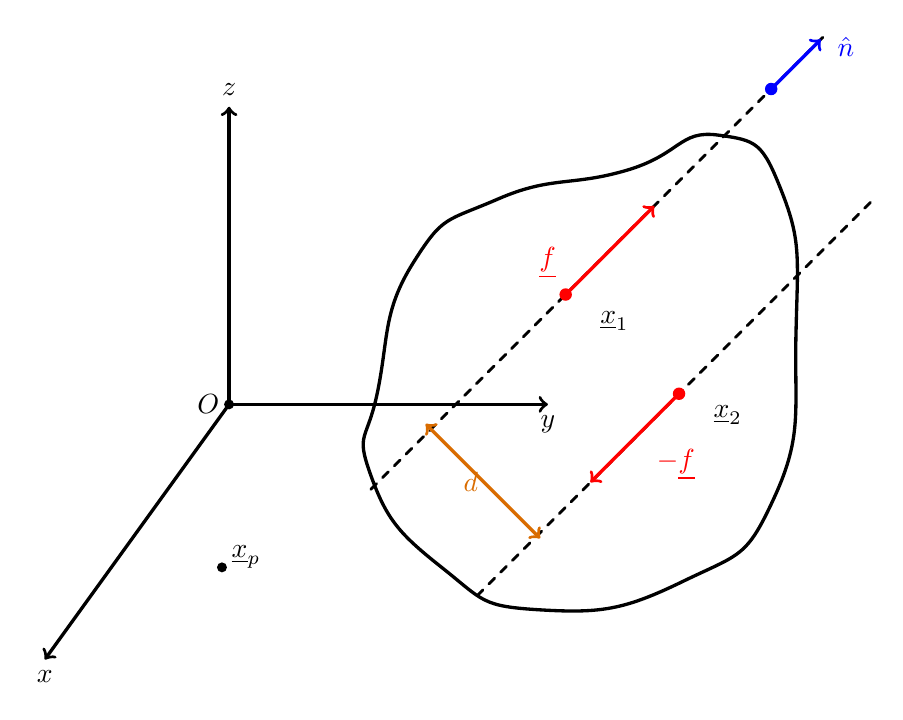
\begin{tikzpicture}[scale=0.9, line cap=round, line join=round]

% Assi
\coordinate (O) at (0,0);
\fill (O) circle (2pt);
\node[left] at (O) {$O$};

\draw[->, very thick] (O) -- (0,4.2) node[above] {$z$};
\draw[->, very thick] (O) -- (4.5,0) node[below] {$y$};
\draw[->, very thick] (O) -- (-2.6,-3.6) node[below] {$x$};

% Punto x_p
\fill (-0.1,-2.3) circle (2pt);
\node[right] at (-0.1,-2.15) {$\underline{x}_p$};

% Contorno del corpo
\draw[very thick]
plot[smooth cycle, tension=0.9] coordinates {
    (2.1,0.2)
    (2.6,2.0)
    (3.8,2.9)
    (5.6,3.3)
    (6.9,3.8)
    (7.8,3.0)
    (8.0,1.0)
    (7.7,-1.3)
    (6.4,-2.5)
    (4.4,-2.9)
    (3.0,-2.3)
    (2.0,-1.0)
};

% Rette parallele tratteggiate
\draw[dashed, line width=1pt] (2.0,-1.2) -- (8.4,5.2);
\draw[dashed, line width=1pt] (3.5,-2.7) -- (9.1,2.9);

% Versore m con punto blu
\fill[blue] (7.65,4.45) circle (2.5pt);
\draw[->, very thick, blue] (7.65,4.45) -- (8.35,5.15);
\node[blue, right] at (8.45,5.05) {$\hat n$};

% Forza superiore
\fill[red] (4.75,1.55) circle (2.5pt);
\draw[->, very thick, red] (4.75,1.55) -- (6,2.8);
\node[red, left] at (4.75,2.0) {$\underline{f}$};
\node[black, below right] at (5.1,1.45) {$\underline{x}_1$};

% Forza inferiore
\fill[red] (6.35,0.15) circle (2.5pt);
\draw[->, very thick, red] (6.35,0.15) -- (5.1,-1.1);
\node[red, right] at (5.9,-0.85) {$-\underline{f}$};
\node[black, right] at (6.7,-0.15) {$\underline{x}_2$};

% Distanza d tra le rette

\draw[<->, very thick, orange!85!black] (4.39, -1.89) -- (2.775 ,  -0.275);
\node[orange!85!black, left] at (3.65,-1.1) {$d$};

\end{tikzpicture}
\end{center}

Calcoliamo il momento delle forze generato dalla coppia di forze rispetto al polo $\underline{x}_p$:
\[
\underline{M}
=
(\underline{x}_1-\underline{x}_p)\wedge f\,\hat n
+
(\underline{x}_2-\underline{x}_p)\wedge (-f\,\hat n)
=
(\underline{x}_1-\underline{x}_2)\wedge f\,\hat n
\]

Quindi il momento generato da una coppia di forze è indipendente dal polo e dipende soltanto dal prodotto dell'intensità della forza e la distanza tra le rette di applicazione. Infatti
\[
\|\underline{M}\| = f\,\|\underline{x}_1-\underline{x}_2\|\sin\alpha = fd
\]

Il vettore $\underline{M}$ è ortogonale al piano su cui giacciono le forze.
È quindi lecito parlare di \textbf{coppia di forze di momento $M$ con verso orario/antiorario}.

\begin{example}{}
Consideriamo un disco che rotola nel piano soggetto ad un momento $M$ orario. Il disco ha massa $m$ e raggio $R$.

\begin{figure}
\centering
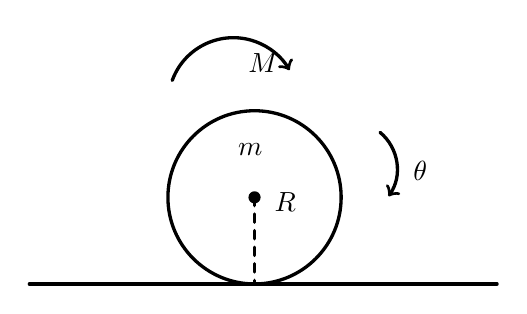
\begin{tikzpicture}[scale=1.1, line cap=round, line join=round]

% Suolo
\draw[very thick] (-2.6,0) -- (2.8,0);

% Disco
\def\R{1.0}
\coordinate (C) at (0,\R);
\draw[very thick] (C) circle (\R);

% Centro e massa
\fill (C) circle (2pt);
\node at (-0.05,1.55) {$m$};

% Raggio tratteggiato
\draw[dashed, very thick] (C) -- (0,0);
\node[right] at (0.12,0.95) {$R$};

% Momento M in senso orario sopra il disco
\draw[->, very thick] (-0.95,2.35) arc[start angle=160,end angle=30,radius=0.75];
\node at (0.1,2.55) {$M$};

% Rotazione theta a destra in senso orario
\draw[->, very thick] (1.45,1.75) arc[start angle=50,end angle=-35,radius=0.55];
\node[right] at (1.72,1.3) {$\theta$};

\end{tikzpicture}
\end{figure}

Applichiamo la seconda legge cardinale scegliendo come polo il punto di contatto $C$:
\[
\frac{d}{dt}\bigl(I_C\omega\bigr)=\sum_{i=1}^{n}(\underline{x}_i-C)\wedge \underline{f}_i
\]

Dal momento che ci è stato dato un momento $\underline{M}$ possiamo supporre che questo venga generato da una coppia di forze parallele e quindi il suo valore sia indipendente dal polo scelto:
\[
\underline{M}
=
\sum_{i=1}^{n}(\underline{x}_i-\underline{x}_p)\wedge \underline{f}_i
=
(\underline{x}_1-\underline{x}_p)\wedge \underline{f}
+
(\underline{x}_2-\underline{x}_p)\wedge (-\underline{f})
\qquad \forall\,\underline{x}_p.
\]

In particolare, scegliendo $\underline{x}_p=C$ e ricordando che per il teorema di Huygens-Steiner il momento d'inerzia di un disco rispetto al punto di contatto è $I_C = I_G + mR^2 = \frac{1}{2}mR^2 + mR^2 = \frac{3}{2}mR^2$, possiamo scrivere:
\[
\frac{d}{dt}\left(\frac{3}{2}mR^2\dot{\theta}\right)=M
\qquad \Longrightarrow \qquad
\frac{3}{2}mR^2\ddot{\theta}=M
\]
\end{example}
\section{Il Teorema di Huygens}

Il seguente teorema è utile per corpi rigidi che ruotano attorno a punti o
assi fissi. Enunciamo e dimostriamo una versione del teorema per moti piani.
\begin{theorem}{}[Teorema di Huygens]
Consideriamo un corpo rigido nel piano che ruota attorno ad un punto fisso
\(\underline{x}_p\). Allora la seconda equazione cardinale rispetto al polo
\(\underline{x}_p\) si scrive nella forma
\[
\frac{d}{dt}\bigl(I_p\underline{\omega}\bigr)
=
\sum_{i=1}^{n} (\underline{x}_i-\underline{x}_p)\wedge \underline{f}_i^{\mathrm{ext}}
\]
con
\[
I_p=I_G+ma^2,
\qquad
a^2=\|\underline{x}_p-\underline{x}_G\|^2.
\]
\end{theorem}

\begin{proof}
Scriviamo la seconda equazione cardinale rispetto al polo \(\underline{x}_p\)
\[
\frac{d}{dt}\Bigl((\underline{x}_G-\underline{x}_p)\wedge m\underline{v}_G+I_G\underline{\omega}\Bigr)
=
\sum_{i=1}^{n} (\underline{x}_i-\underline{x}_p)\wedge \underline{f}_i^{\mathrm{ext}}
-
\underline{v}_p\wedge m\underline{v}_G.
\]

Notiamo che \(\underline{v}_p=\underline{0}\), quindi
\[
-\underline{v}_p\wedge m\underline{v}_G=\underline{0}.
\]

Inoltre uso la formula fondamentale della cinematica per \(\underline{x}_p\) e
\(\underline{x}_G\)
\[
\underline{v}_G=\underline{v}_p+\underline{\omega}\wedge(\underline{x}_G-\underline{x}_p)
=
\underline{\omega}\wedge(\underline{x}_G-\underline{x}_p).
\]

Sostituendo si ottiene
\[
\frac{d}{dt}\Bigl((\underline{x}_G-\underline{x}_p)\wedge
m\bigl(\underline{\omega}\wedge(\underline{x}_G-\underline{x}_p)\bigr)
+
I_G\underline{\omega}\Bigr)
=
\sum_{i=1}^{n} (\underline{x}_i-\underline{x}_p)\wedge \underline{f}_i^{\mathrm{ext}}.
\]

Uso la formula
\[
\underline{a}\wedge(\underline{b}\wedge \underline{a})
=
\underline{b}\,(\underline{a}\cdot \underline{a})
-
\underline{a}\,(\underline{a}\cdot \underline{b})
\]
con
\[
\underline{a}=\underline{x}_G-\underline{x}_p,
\qquad
\underline{b}=m\underline{\omega}.
\]
Allora
\[
(\underline{x}_G-\underline{x}_p)\wedge
m\bigl(\underline{\omega}\wedge(\underline{x}_G-\underline{x}_p)\bigr)
=
m\underline{\omega}\,\|\underline{x}_G-\underline{x}_p\|^2
-
(\underline{x}_G-\underline{x}_p)\bigl(m\underline{\omega}\cdot(\underline{x}_G-\underline{x}_p)\bigr).
\]
Poiché \(\underline{\omega}\perp(\underline{x}_G-\underline{x}_p)\), il secondo
termine si annulla e quindi
\[
(\underline{x}_G-\underline{x}_p)\wedge
m\bigl(\underline{\omega}\wedge(\underline{x}_G-\underline{x}_p)\bigr)
=
m\underline{\omega}\,\|\underline{x}_G-\underline{x}_p\|^2.
\]

Allora
\[
\frac{d}{dt}\Bigl(m\|\underline{x}_G-\underline{x}_p\|^2\underline{\omega}
+
I_G\underline{\omega}\Bigr)
=
\sum_{i=1}^{n} (\underline{x}_i-\underline{x}_p)\wedge \underline{f}_i^{\mathrm{ext}}.
\]

Imponendo
\[
I_p=m\|\underline{x}_G-\underline{x}_p\|^2+I_G
\]
otteniamo
\[
\frac{d}{dt}\bigl(I_p\underline{\omega}\bigr)
=
\sum_{i=1}^{n} (\underline{x}_i-\underline{x}_p)\wedge \underline{f}_i^{\mathrm{ext}}.
\]
\end{proof}


\section{Esempi applicativi}
\begin{example}{}
Consideriamo un'asta con un estremo fissato, massa \(m\) e lunghezza \(\ell\).

\begin{figure}
\centering
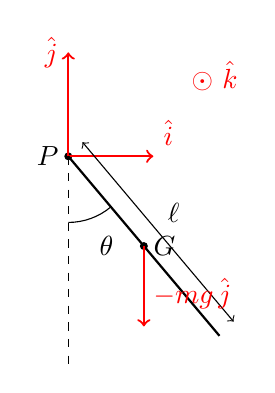
\begin{tikzpicture}[scale=1.2]
    % punto P
    \fill (0,0) circle (1.2pt);
    \node[left] at (0,0) {\(P\)};

    % assi
    \draw[red,->,thick] (0,0) -- (0.9,0) node[above right] {\(\hat{i}\)};
    \draw[red,->,thick] (0,0) -- (0,1.1) node[left] {\(\hat{j}\)};
    \node[red] at (1.55,0.85) {\(\odot\ \hat{k}\)};

    % verticale tratteggiata
    \draw[dashed] (0,0) -- (0,-2.2);

    % asta
    \draw[thick] (0,0) -- (1.6,-1.9);
    \draw[<->] (0.15,0.15) -- node[above right] {\(\ell\)} (1.75,-1.75);

    % centro di massa G
    \fill (0.8,-0.95) circle (1.2pt);
    \node[right] at (0.8,-0.95) {\(G\)};

    % forza peso
    \draw[red,->,thick] (0.8,-0.95) -- (0.8,-1.8);
    \node[right,red] at (0.8,-1.45) {\(-mg\,\hat{j}\)};

    % angolo theta
    \draw (0,-0.7) arc[start angle=-90,end angle=-50,radius=0.7];
    \node[left] at (0.58,-0.95) {\(\theta\)};
\end{tikzpicture}
\end{figure}

Imponiamo i vincoli
\[
\underline{x}_p=(k_1,k_2,0).
\]
Il sistema ha quindi \(3-2=1\) grado di libertà. Scriviamo la seconda legge
cardinale rispetto al polo \(p\):
\[
\frac{d}{dt}\bigl(I_p\dot{\theta}\bigr)
=
\frac{d}{dt}\bigl((I_G+ma^2)\dot{\theta}\bigr)
=
\frac{d}{dt}\left(\left(\frac{m\ell^2}{12}+m\left(\frac{\ell}{2}\right)^2\right)\dot{\theta}\right)
=
(\underline{x}_G-\underline{x}_p)\wedge(-mg\,\hat{j}).
\]

\[
\Rightarrow\quad
\frac{d}{dt}\left(\left(\frac{m\ell^2}{12}+\frac{m\ell^2}{4}\right)\dot{\theta}\right)
=
-\frac{\ell}{2}\,mg\,\sin(\pi-\theta)\,\hat{k}
=
-\frac{\ell}{2}\,mg\,\sin\theta\,\hat{k}.
\]

\[
\Rightarrow\quad
\frac{d}{dt}\left(\frac{m\ell^2}{3}\dot{\theta}\right)
=
-\frac{\ell}{2}\,mg\,\sin\theta
\Rightarrow
\frac{\ell}{3}\ddot{\theta}
=
-\frac{g}{2}\sin\theta
\Rightarrow
\ddot{\theta}
=
-\frac{3}{2}\frac{g}{\ell}\sin\theta.
\]

L'ultima equazione differenziale si risolve con il metodo delle funzioni
ellittiche.

Notiamo che la soluzione \(\theta(t)\) non può dipendere dalla massa.

Sotto l'ipotesi delle piccole oscillazioni \(\left(\theta\ll \frac{\pi}{2}\right)\)
allora
\[
\sin\theta=\theta+o(\theta^2),
\]
cioè possiamo linearizzare il problema:
\[
\ddot{\theta}
=
-\frac{3}{2}\frac{g}{\ell}\theta,
\qquad
\omega^2=\frac{3}{2}\frac{g}{\ell}
\]
\[
\Rightarrow\quad
\ddot{\theta}+\omega^2\theta=0
\Rightarrow
\lambda^2+\omega^2=0
\Rightarrow
\lambda=\pm i\omega.
\]

\[
\Rightarrow\quad
\theta(t)=A\cos(\omega t+\varphi),
\qquad
A \text{ e } \varphi \text{ fissate dalle condizioni iniziali.}
\]


\begin{oss}{}
Avremmo potuto ricavare \(\theta(t)\) anche attraverso la prima equazione
cardinale. Partiamo da
\[
\begin{cases}
x_G=\dfrac{\ell}{2}\sin\theta\\[4pt]
y_G=-\dfrac{\ell}{2}\cos\theta
\end{cases}
\qquad \Rightarrow \qquad
\begin{cases}
v_G^x=\dot{\theta}\,\dfrac{\ell}{2}\cos\theta\\[4pt]
v_G^y=\dot{\theta}\,\dfrac{\ell}{2}\sin\theta
\end{cases}
\qquad \Rightarrow \qquad
\begin{cases}
a_G^x=\dfrac{\ell}{2}\cos\theta\,\ddot{\theta}-\dfrac{\ell}{2}\sin\theta\,\dot{\theta}^2\\[4pt]
a_G^y=\dfrac{\ell}{2}\sin\theta\,\ddot{\theta}+\dfrac{\ell}{2}\cos\theta\,\dot{\theta}^2
\end{cases}
\]

\[
\Rightarrow
\begin{cases}
m\left[\dfrac{\ell}{2}\cos\theta\,\ddot{\theta}-\dfrac{\ell}{2}\sin\theta\,\dot{\theta}^2\right]=R_x\\[8pt]
m\left[\dfrac{\ell}{2}\sin\theta\,\ddot{\theta}+\dfrac{\ell}{2}\cos\theta\,\dot{\theta}^2\right]=-mg+R_y
\end{cases}
\]

dove
\[
\underline{R}=R_x\hat{i}+R_y\hat{j}
\]
è la reazione vincolare dovuta al vincolo in \(\underline{x}_p\), il cui momento
rispetto a \(\underline{x}_p\) è nullo e che quindi abbiamo ignorato nei calcoli
precedenti.

Se al sistema di equazioni che abbiamo trovato aggiungiamo
\[
\frac{d}{dt}\bigl(I_G\dot{\theta}\bigr)=-\underline{x}_G\wedge \underline{R}
\qquad \Longleftrightarrow \qquad
\frac{d}{dt}\left(\frac{m\ell^2}{12}\dot{\theta}\,\hat{k}\right)
=
-\left[\frac{\ell}{2}R_x\cos\theta+\frac{\ell}{2}R_y\sin\theta\right]\hat{k}
\]
otteniamo \(3\) equazioni indipendenti per le \(3\) incognite scalari
\(\theta\), \(R_x\), \(R_y\).

È indubbiamente evidente la facilità del primo procedimento rispetto a
quest'ultimo.
\end{oss}

\end{example}


\begin{example}{}
Consideriamo un disco di massa \(m\) e raggio \(R\) vincolato a muoversi
in un piano verticale. Al centro di massa del disco è attaccata una
molla a riposo. Il disco si muove di puro rotolamento rispetto al
terreno. Sia \(K\) la costante elastica della molla.

\begin{figure}
\centering
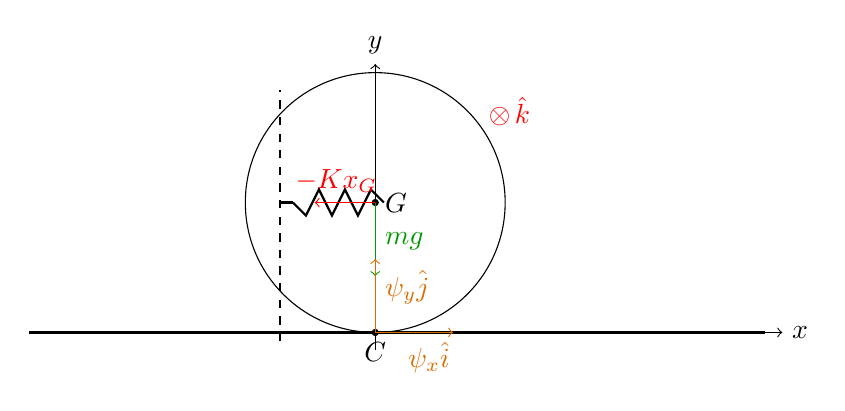
\begin{tikzpicture}[scale=1.1]
    % terreno
    \draw[thick] (-4,0) -- (4.5,0);
    \draw[->] (0,0) -- (4.7,0) node[right] {\(x\)};

    % asse y
    \draw[->] (0,-0.2) -- (0,3.1) node[above] {\(y\)};

    % disco
    \draw (0,1.5) circle (1.5);

    % centro e punto di contatto
    \fill (0,1.5) circle (1.2pt);
    \node[right] at (0,1.5) {\(G\)};
    \fill (0,0) circle (1.2pt);
    \node[below] at (0,0) {\(C\)};

    % linea tratteggiata
    \draw[dashed] (-1.1,-0.1) -- (-1.1,2.8);

    % molla
    \draw[thick] (-1.1,1.5) -- (-0.95,1.5);
    \draw[thick] (-0.95,1.5) -- (-0.8,1.35) -- (-0.65,1.65) -- (-0.5,1.35) -- (-0.35,1.65) -- (-0.2,1.35) -- (-0.05,1.65) -- (0.1,1.5);

    % versore k entrante
    \node[red] at (1.55,2.55) {\(\otimes\,\hat{k}\)};

    % forza elastica
    \draw[red,->] (0,1.5) -- (-0.7,1.5);
    \node[red,above] at (-0.45,1.5) {\(-Kx_G\)};

    % peso
    \draw[green!60!black,->] (0,1.5) -- (0,0.65);
    \node[green!60!black,right] at (0,1.05) {\(mg\)};

    % reazioni vincolari
    \draw[orange!85!black,->] (0,0) -- (0.9,0);
    \node[orange!85!black,below] at (0.62,0) {\(\psi_x\hat{i}\)};

    \draw[orange!85!black,->] (0,0) -- (0,0.85);
    \node[orange!85!black,right] at (0,0.52) {\(\psi_y\hat{j}\)};
\end{tikzpicture}
\end{figure}

Impongo i vincoli di puro rotolamento
\[
\underline{v}_C=\underline{0}
\quad \Rightarrow \quad
v_C^x=v_C^y=0
\quad \Rightarrow \quad
\text{il sistema ha } 3-2=1 \text{ grado di libertà.}
\]

In un moto di puro rotolamento vale
\[
\dot{x}_G=R\dot{\theta}
\quad \Rightarrow \quad
x_G=R\theta+C.
\]
Per la nostra configurazione \(C=0\).

Impostiamo la prima legge cardinale
\[
\begin{cases}
m\ddot{x}_G=-Kx_G+\psi_x,\\[4pt]
m\ddot{y}_G=-mg+\psi_y.
\end{cases}
\]

Dal momento che le forze lungo \(\hat{j}\) sono parallele al braccio non c'è
momento. Lo stesso vale per la forza elastica che ha braccio nullo.
Nella seconda equazione cardinale rispetto a \(G\) rimane solo
\[
(\underline{x}_C-\underline{x}_G)\wedge \psi_x\hat{i}
=
-R\psi_x\hat{k}
\quad \Rightarrow \quad
\frac{d}{dt}\bigl(I_G\dot{\theta}\bigr)=-R\psi_x.
\]

Dobbiamo quindi risolvere il sistema
\[
\begin{cases}
m\ddot{x}_G=-Kx_G+\psi_x,\\[4pt]
m\ddot{y}_G=-mg+\psi_y,\\[4pt]
\dfrac{d}{dt}\bigl(I_G\dot{\theta}\bigr)=-R\psi_x.
\end{cases}
\]

Ma
\[
x_G=R\theta,\qquad \ddot{y}_G=0,\qquad I_G=\frac{mR^2}{2}
\]
e quindi
\[
\begin{cases}
mR\ddot{\theta}=-KR\theta+\psi_x,\\[4pt]
0=-mg+\psi_y,\\[4pt]
\dfrac{mR}{2}\ddot{\theta}=-R\psi_x.
\end{cases}
\]

Sistema di \(3\) equazioni nelle \(3\) incognite \(\psi_x,\psi_y,\theta\).
\end{example}


\begin{example}{}
Consideriamo un'asta di lunghezza \(\ell\) e massa \(m\) collegata all'estremo
superiore ad una molla di costante elastica \(K\).
\begin{center}
\begin{tikzpicture}[scale=1.1, >=stealth]
    % assi
    \draw[->,line width=1.2pt] (0,0) -- (4.5,0) node[right] {$x$};
    \draw[->,line width=1.2pt] (0,0) -- (0,5.8) node[above] {$y$};

    % Punti calcolati con terna pitagorica 3-4-5 per un rigore matematico assoluto!
    % Lunghezza asta = 5, quota soffitto \ell = 5
    \coordinate (A) at (0,4);
    \coordinate (B) at (3,0);
    \coordinate (G) at ($(A)!0.5!(B)$);
    \coordinate (S1) at (0,5); % Soffitto a quota 5

    % quota \ell (altezza 5)
    \draw[line width=1.2pt] (-1.55,0) -- (-1.55,5.0);
    \draw[line width=1.2pt] (-1.75,0) -- (-1.35,0);
    \draw[line width=1.2pt] (-1.75,5.0) -- (-1.35,5.0);
    \node[left] at (-1.55,2.5) {$\ell$};

    % guida verticale in A
    \draw[line width=1.3pt] (-0.15,4.2) -- (-0.15,3.8);
    \draw[line width=1.3pt] ( 0.15,4.2) -- ( 0.15,3.8);

    % guida orizzontale in B
    \draw[line width=1.3pt] (2.8, 0.15) -- (3.2, 0.15);
    \draw[line width=1.3pt] (2.8,-0.15) -- (3.2,-0.15);

    % asta
    \draw[line width=1.4pt] (A) -- (B);

    % molla disegnata a zig-zag proporzionato tra Soffitto(5.0) e A(4.0)
    \fill (S1) circle (2.2pt);
    \draw[line width=1.2pt] (S1) -- (0,4.85) -- (-0.12,4.7) -- (0.12,4.55) -- (-0.12,4.4) -- (0.12,4.25) -- (0,4.1) -- (A);

    % punti A, B, G
    \fill (A) circle (2pt);
    \fill (B) circle (2pt);
    \fill[red] (G) circle (2pt);

    \node[left] at (A) {$A$};
    \node[below] at (B) {$B$};

    % forze attive
    \draw[->,red,line width=1.1pt] (A) -- ++(0,0.85);
    \node[red,right] at ($(A)+(0.05,0.6)$) {$\underline{F}_{el}$};

    \draw[->,red,line width=1.1pt] (G) -- ++(0,-1.0);
    \node[red,right] at ($(G)+(0.15,-0.5)$) {$m\underline{g}$};

    % reazioni vincolari incognite
    \draw[->,green!60!black,line width=1.1pt] (A) -- ++(1.4,0);
    \node[green!60!black,above] at ($(A)+(1.0,0)$) {$\underline{\psi}$};

    \draw[->,green!60!black,line width=1.1pt] (B) -- ++(0,1.25);
    \node[green!60!black,right] at ($(B)+(0,0.75)$) {$\underline{\varphi}$};

    % angolo theta: posizionato e calcolato in modo esatto
    % Con i cateti a 3 e 4, l'angolo d'inclinazione è di circa 53.13 gradi
    \draw[->,line width=0.9pt] (0,2.8) arc[start angle=-90,end angle=-53.13,radius=1.2];
    \node at (0.45, 2.5) {$\theta$};

    % versore k uscente
    \node[red] at (3.5,4.8) {$\odot\,\hat{k}$};

\end{tikzpicture}
\end{center}


L'asta è soggetta ai vincoli
\[
x_A=0,\qquad y_B=0
\]
e ha quindi \(3-2=1\) grado di libertà. Inoltre la molla è a riposo per
\(\theta=0\). Scegliamo \(\theta(t)\) come coordinata libera.

Le forze attive sono
\[
\underline{F}_{el}=K(\ell-\ell\cos\theta)\,\hat{j},
\qquad
-mg\,\hat{j}.
\]

Le forze vincolari incognite sono \(\psi\,\hat{i}\) applicata in \(A\) e
\(\varphi\,\hat{j}\) applicata in \(B\).

Impostiamo la prima equazione cardinale
\[
\frac{d}{dt}\bigl(m\underline{v}_G\bigr)=\sum_{i=1}^{n}\underline{f}_i^{\mathrm{ext}}.
\]

Poiché
\[
\begin{cases}
x_G=\dfrac{\ell}{2}\sin\theta,\\[4pt]
y_G=\dfrac{\ell}{2}\cos\theta,
\end{cases}
\qquad \Rightarrow \qquad
\begin{cases}
\dot{x}_G=\dfrac{\ell}{2}\cos\theta\,\dot{\theta},\\[4pt]
\dot{y}_G=-\dfrac{\ell}{2}\sin\theta\,\dot{\theta},
\end{cases}
\]
si ha
\[
\begin{cases}
\ddot{x}_G=\dfrac{\ell}{2}\bigl(\cos\theta\,\ddot{\theta}-\sin\theta\,\dot{\theta}^{2}\bigr),\\[6pt]
\ddot{y}_G=-\dfrac{\ell}{2}\bigl(\sin\theta\,\ddot{\theta}+\cos\theta\,\dot{\theta}^{2}\bigr).
\end{cases}
\]

Allora otteniamo
\[
\begin{cases}
\psi(t)=m\ddot{x}_G
=
m\,\dfrac{\ell}{2}\bigl(\cos\theta\,\ddot{\theta}-\sin\theta\,\dot{\theta}^{2}\bigr),\\[10pt]
-mg+K(\ell-\ell\cos\theta)+\varphi
=
m\ddot{y}_G
=
-\,m\,\dfrac{\ell}{2}\bigl(\sin\theta\,\ddot{\theta}+\cos\theta\,\dot{\theta}^{2}\bigr).
\end{cases}
\]

Da cui
\[
\varphi(t)
=
-\,m\,\frac{\ell}{2}\bigl(\sin\theta\,\ddot{\theta}+\cos\theta\,\dot{\theta}^{2}\bigr)
+mg-K\ell(1-\cos\theta).
\]

Serve determinare \(\theta(t)\). Proviamo a farlo tramite la seconda equazione
cardinale con polo in \(G\):
\[
\frac{d}{dt}\bigl(I_G\dot{\theta}\bigr)
=
\sum_{i=1}^{n}(\underline{x}_i-\underline{x}_G)\wedge \underline{f}_i^{\mathrm{ext}},
\qquad
I_G=\frac{m\ell^{2}}{12}.
\]

Quindi
\[
\frac{m\ell^{2}}{12}\,\ddot{\theta}\,\hat{k}
=
(\underline{x}_A-\underline{x}_G)\wedge K\ell(1-\cos\theta)\,\hat{j}
+
(\underline{x}_A-\underline{x}_G)\wedge \psi\,\hat{i}
+
(\underline{x}_B-\underline{x}_G)\wedge \varphi\,\hat{j}.
\]

Ovvero
\[
\frac{m\ell^{2}}{12}\,\ddot{\theta}
=
-\,\frac{\ell}{2}\,K\ell(1-\cos\theta)\sin(2\pi-\theta)
-\,\frac{\ell}{2}\,\psi\sin\!\left(\frac{3}{2}\pi-\theta\right)
+\,\frac{\ell}{2}\,\varphi\sin(\pi-\theta),
\]
cioè
\[
\frac{m\ell^{2}}{12}\,\ddot{\theta}
=
-\,\frac{\ell}{2}\,K\ell(1-\cos\theta)\sin\theta
+\,\frac{\ell}{2}\,\psi\cos\theta
+\,\frac{\ell}{2}\,\varphi\sin\theta.
\]

A questo punto dovremmo sostituire \(\varphi(t)\) e \(\psi(t)\) e trovare
\(\theta(t)\), ma diventa complesso. Cerchiamo un polo diverso.

Alla fine della lezione sul teorema di Mozzi avevamo trovato il centro di
istantanea rotazione del sistema
\[
\underline{x}_D=x_B\,\hat{i}+y_A\,\hat{j}.
\]

\begin{tikzpicture}[scale=1.15]
    % punti
    \coordinate (O) at (0,0);
    \coordinate (A) at (0,3.2);
    \coordinate (B) at (5.2,0);
    \coordinate (D) at (5.2,3.2);
    \coordinate (G) at ($(A)!0.5!(B)$);

    % assi
    \draw[->,line width=1.2pt] (-1.8,0) -- (7.0,0) node[right] {$x$};
    \draw[->,line width=1.2pt] (0,-0.6) -- (0,5.0);

    % asta e diagonale
    \draw[line width=1.3pt] (A) -- (B);
    \draw[line width=1.3pt] (O) -- (D);

    % tratteggi
    \draw[dashed,line width=1pt] (A) -- (D);
    \draw[dashed,line width=1pt] (D) -- (B);

    % punti
    \fill (A) circle (2pt);
    \fill (B) circle (2pt);
    \fill (D) circle (2pt);
    \fill[red] (G) circle (2pt);

    % etichette
    \node[left] at (A) {$A$};
    \node[below] at (B) {$B$};
    \node[above right] at (D) {$D$};
    \node[below] at (G) {$G$};

    % forza elastica
    \draw[->,red,line width=1.1pt] (A) -- ++(0,1.2);
    \node[red,right] at ($(A)+(0.05,0.95)$) {$\underline{F}_e$};

    % reazione psi in A
    \draw[->,green!60!black,line width=1.1pt] (A) -- ++(1.25,0);
    \node[green!60!black,above] at ($(A)+(0.9,0)$) {$\psi$};

    % reazione phi in B
    \draw[->,green!60!black,line width=1.1pt] (B) -- ++(0,1.25);
    \node[green!60!black,right] at ($(B)+(0,0.85)$) {$\varphi$};

    % peso in G
    \draw[->,red,line width=1.1pt] (G) -- ++(0,-1.1);

    % angolo theta
    \draw[->,line width=0.9pt] (0,2.45) arc[start angle=270,end angle=325,radius=0.75];
    \node at (0.62,1.7) {$\theta$};

    % scritta l/2
    \node at (3.95,1.95) {$\ell/2$};

    % versore k uscente
    \node[red] at (3.7,4.2) {$\odot\,\hat{k}$};
\end{tikzpicture}
\\Scriviamo la seconda equazione cardinale rispetto a \(D\):
\[
\frac{d}{dt}\Bigl((\underline{x}_G-\underline{x}_D)\wedge m\underline{v}_G
+I_G\underline{\omega}\Bigr)
=
(\underline{x}_B-\underline{x}_D)\wedge \varphi\,\hat{j}
+
(\underline{x}_A-\underline{x}_D)\wedge \psi\,\hat{i}
\]
\[
\qquad
+
(\underline{x}_A-\underline{x}_D)\wedge K\ell(1-\cos\theta)\,\hat{j}
+
(\underline{x}_G-\underline{x}_D)\wedge (-mg\,\hat{j})
-
\underline{v}_D\wedge m\underline{v}_G.
\]

Utilizziamo
\[
\underline{v}_G=\underline{\omega}\wedge(\underline{x}_G-\underline{x}_D)
\]
nel primo membro:
\[
\frac{d}{dt}\Bigl((\underline{x}_G-\underline{x}_D)\wedge
m\bigl(\underline{\omega}\wedge(\underline{x}_G-\underline{x}_D)\bigr)
+I_G\underline{\omega}\Bigr)
=
\frac{d}{dt}\Bigl(m\|\underline{x}_G-\underline{x}_D\|^{2}\underline{\omega}
+I_G\underline{\omega}\Bigr).
\]

Quindi
\[
\frac{d}{dt}\Bigl[\bigl(I_G+m\|\underline{x}_G-\underline{x}_D\|^{2}\bigr)
\dot{\theta}\,\hat{k}\Bigr]
=
\frac{d}{dt}\Bigl[\left(\frac{m\ell^{2}}{12}+m\left(\frac{\ell}{2}\right)^{2}\right)
\dot{\theta}\,\hat{k}\Bigr]
\]
\[
=
-\,\ell\sin\theta\cdot K\ell(1-\cos\theta)\,\hat{k}
+
\frac{\ell}{2}mg\sin\theta\,\hat{k}.
\]

Pertanto
\[
\frac{m\ell^{2}}{3}\,\ddot{\theta}
=
-\,K\ell^{2}\sin\theta(1-\cos\theta)
+
\frac{\ell}{2}mg\sin\theta.
\]

Questa equazione non si può risolvere analiticamente ma va risolta in modo
numerico.
\end{example}
